\documentclass[aspectratio=169]{beamer}
\usepackage{tikz}
\usetikzlibrary{shapes.geometric}
\usetikzlibrary{positioning}
\usetikzlibrary{arrows.meta}
\usepackage{amsmath}
\usepackage{pgfplots}
\usepackage{listings}
\usepackage{xcolor}
\pgfplotsset{compat=1.16}

% Theme and color settings
\usetheme{Madrid}
\usecolortheme{default}
\definecolor{codegreen}{RGB}{0,128,0}
\definecolor{codegray}{RGB}{128,128,128}
\definecolor{codepurple}{RGB}{128,0,128}
\definecolor{backcolour}{RGB}{245,245,245}
\definecolor{tabserablue}{RGB}{0,51,102}
\definecolor{lightgray}{RGB}{240,240,240}

% Code listing style
\lstdefinestyle{mystyle}{
    backgroundcolor=\color{backcolour},   
    commentstyle=\color{codegreen},
    keywordstyle=\color{blue},
    numberstyle=\tiny\color{codegray},
    stringstyle=\color{codepurple},
    basicstyle=\ttfamily\footnotesize,
    breakatwhitespace=false,         
    breaklines=true,                 
    captionpos=b,                    
    keepspaces=true,                 
    numbers=left,                    
    numbersep=5pt,                  
    showspaces=false,                
    showstringspaces=false,
    showtabs=false,                  
    tabsize=2
}
\lstset{style=mystyle}

% Conditional logo overlay
\IfFileExists{tabsera.png}{%
    \addtobeamertemplate{background canvas}{}{%
        \begin{tikzpicture}[remember picture,overlay]
            \node[anchor=north east,inner sep=5pt] at (current page.north east) {
                \includegraphics[height=0.6cm]{tabsera.png}
            };
        \end{tikzpicture}
    }
    \addtobeamertemplate{frametitle}{}{%
        \begin{tikzpicture}[remember picture,overlay]
            \node[anchor=north east,inner sep=5pt] at (current page.north east) {
                \includegraphics[height=0.6cm]{tabseraw.png}
            };
        \end{tikzpicture}
    }
}{}

\setbeamertemplate{footline}{%
    \leavevmode%
    \hbox{%
        \begin{beamercolorbox}[wd=.333333\paperwidth,ht=2.25ex,dp=1ex,center]{author in head/foot}%
            \usebeamerfont{author in head/foot}TABSERA Education
        \end{beamercolorbox}%
        \begin{beamercolorbox}[wd=.333333\paperwidth,ht=2.25ex,dp=1ex,center]{title in head/foot}%
            \usebeamerfont{title in head/foot}IGCSE Learning Strategies
        \end{beamercolorbox}%
        \begin{beamercolorbox}[wd=.333333\paperwidth,ht=2.25ex,dp=1ex,right]{date in head/foot}%
            \usebeamerfont{date in head/foot}\insertframenumber{} / \inserttotalframenumber\hspace*{2ex}
        \end{beamercolorbox}%
    }%
    \vskip0pt%
}

\begin{document}

% ═══════════════════════════════════════════════════════════════
% SLIDE 1: TITLE SLIDE
% ═══════════════════════════════════════════════════════════════
\begin{frame}[t]
\begin{center}
{\Huge The Night Before and Exam Day Protocols}

\vspace{0.3cm}

{\Large Tabsera Academy IGCSE Learning Strategies Course}

\vspace{0.2cm}

{\large Lesson 4.4 | Exam Excellence | ✍️ Exam Skills}

\vspace{0.3cm}

\IfFileExists{lesson4-4-1-1.png}{%
    \includegraphics[width=0.25\textwidth]{lesson4-4-1-1.png}
}{}

\vspace{0.2cm}

{\small TABSERA Education | Achieving A* Across 7 IGCSE Subjects}
\end{center}
\end{frame}

% Voice Script for Slide 1:
% "Welcome to Tabsera Academy IGCSE Learning Strategies Course, lesson 4.4: The Night Before and Exam Day Protocols. This lesson is part of Unit 4, focusing on Exam Excellence. Today we'll explore essential exam skills that apply to all seven IGCSE subjects. Many students lose marks not because they don't know the content, but because they mismanage the critical 24 hours before and during exams. Research shows that proper exam day protocols can improve performance by up to 15 percent. Whether you're facing Chemistry Paper 2 with its 508 lessons of content, Physics calculations, or Mathematics problem-solving, these protocols will help you perform at your absolute best when it matters most. Let's begin developing these powerful exam-day strategies together."

% GPT Image Prompt for lesson4-4-1-1.png:
% "Professional IGCSE exam preparation illustration showing diverse international student aged 14-16 confidently preparing for exams, organized exam materials and checklist visible, calm and focused atmosphere, modern educational setting with IGCSE textbooks, blue and green gradient colors, clean minimalist design suitable for Muslim learners worldwide, academic excellence theme, small compact square illustration. IMPORTANT: If any female figures are shown, they must wear full hijab covering hair completely with modest dress. Show single-gender image only."

% ═══════════════════════════════════════════════════════════════
% SLIDE 2: LEARNING OBJECTIVES
% ═══════════════════════════════════════════════════════════════
\begin{frame}[t]
\frametitle{Learning Objectives}
\fontsize{9pt}{10pt}\selectfont
\begin{columns}[T]
\begin{column}{0.58\textwidth}
\textbf{By the end of this lesson, you will be able to:}
\vspace{0.1cm}

\begin{itemize}
    \item Design optimal pre-exam evening routine for peak performance
    \vspace{0.05cm}
    \item Execute morning preparation checklist for exam readiness
    \vspace{0.05cm}
    \item Apply in-exam protocols for time management and accuracy
    \vspace{0.05cm}
    \item Practice post-exam reflection without compromising future performance
\end{itemize}

\vspace{0.2cm}
\textbf{Focus:} Exam Skills | \textbf{Applies to:} All 7 Subjects
\end{column}

\begin{column}{0.38\textwidth}
\IfFileExists{lesson4-4-2-1.png}{%
    \includegraphics[width=0.95\textwidth,keepaspectratio]{lesson4-4-2-1.png}
}{}
\end{column}
\end{columns}
\end{frame}

% Voice Script for Slide 2:
% "Let's look at what you'll accomplish in this lesson. First, you'll design an optimal pre-exam evening routine that prepares your mind and body for peak performance. Second, you'll create a morning preparation checklist ensuring you arrive at the exam room ready and confident. Third, you'll master in-exam protocols for managing time effectively and maximizing accuracy across all question types. Finally, you'll learn post-exam reflection techniques that help future performance without causing unnecessary stress. These aren't just theoretical concepts - they're battle-tested protocols used by thousands of successful IGCSE students. By mastering these exam-day skills, you'll approach Chemistry practicals, Physics calculations, Mathematics problems, and all other subjects with confidence and control."

% GPT Image Prompt for lesson4-4-2-1.png:
% "Educational illustration of study goals and exam objectives, diverse international teenager aged 14-16 with clear learning targets and exam checklist visible, motivational study environment, IGCSE exam papers and organized materials, confident expression, modern workspace with calendar showing exam dates, blue and green colors, professional quality, suitable for Muslim learners. IMPORTANT: If any female figures are shown, they must wear full hijab covering hair completely with modest dress. Show single-gender image only."

% ═══════════════════════════════════════════════════════════════
% SLIDE 3: THE CHALLENGE
% ═══════════════════════════════════════════════════════════════
\begin{frame}[t]
\frametitle{The Challenge: Common Exam Day Mistakes}
\fontsize{9pt}{10pt}\selectfont
\begin{columns}[T]
\begin{column}{0.58\textwidth}

\textbf{Many IGCSE students struggle with:}
\vspace{0.1cm}

\begin{itemize}
    \item \textbf{Problem 1:} Cramming new content night before exam
    \vspace{0.05cm}
    \item \textbf{Problem 2:} Poor sleep leading to mental fatigue
    \vspace{0.05cm}
    \item \textbf{Problem 3:} Arriving rushed, stressed, or unprepared
    \vspace{0.05cm}
    \item \textbf{Result:} Preventable mistakes, time pressure, underperformance
\end{itemize}

\vspace{0.2cm}
\textbf{The Solution:} Evidence-based protocols eliminate these problems completely.
\end{column}

\begin{column}{0.38\textwidth}
\IfFileExists{lesson4-4-3-1.png}{%
    \includegraphics[width=0.95\textwidth,keepaspectratio]{lesson4-4-3-1.png}
}{}
\end{column}
\end{columns}
\end{frame}

% Voice Script for Slide 3:
% "Before we dive into solutions, let's understand why exam day protocols matter. Many IGCSE students make the critical mistake of cramming new Chemistry equations or Physics formulas the night before their exam. Research shows this actually impairs memory consolidation and increases anxiety. Another common problem is sacrificing sleep to study more - but cognitive science proves that sleep deprivation reduces exam performance by up to 20 percent. Perhaps worst of all, students arrive at the exam room rushed, having forgotten essential equipment or not eaten properly, starting with immediate disadvantage. These problems are completely preventable. The protocols we're learning today are based on research from cognitive psychology and proven by thousands of successful IGCSE students achieving A* grades. Let's eliminate these mistakes forever."

% GPT Image Prompt for lesson4-4-3-1.png:
% "Educational illustration showing exam stress and common mistakes, student surrounded by too many textbooks cramming late at night, tired expression with clock showing late hour, scattered exam materials, stressed but hopeful atmosphere, modern setting, blue and orange colors indicating challenge then solution, professional quality, suitable for Muslim learners. IMPORTANT: If any female figures are shown, they must wear full hijab covering hair completely with modest dress. Show single-gender image only."

% ═══════════════════════════════════════════════════════════════
% SLIDE 4: CORE STRATEGY 1 - The Night Before Protocol
% ═══════════════════════════════════════════════════════════════
\begin{frame}[t]
\frametitle{The Night Before: Optimal Pre-Exam Routine}
\fontsize{9pt}{10pt}\selectfont

\begin{columns}[T]
    \begin{column}{0.48\textwidth}
        \textbf{Evening Protocol (6pm-10pm):}
        \vspace{0.1cm}
        \begin{itemize}
            \item \textbf{6-7pm:} Light review of summary notes only
            \vspace{0.05cm}
            \item \textbf{7-8pm:} Prepare equipment, check exam details
            \vspace{0.05cm}
            \item \textbf{8-10pm:} Relaxation, early sleep (8+ hours)
        \end{itemize}
        
        \vspace{0.2cm}
        \textbf{Why It Works:} Memory consolidation occurs during sleep; stress reduction improves recall.
    \end{column}
    
    \begin{column}{0.48\textwidth}
        \textbf{Evening Timeline:}
        \vspace{0.1cm}
        \begin{center}
        \resizebox{!}{0.60\textwidth}{
        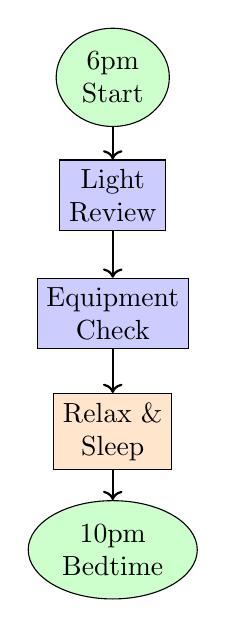
\begin{tikzpicture}[node distance=1.2cm]
            \node[draw, ellipse, fill=green!20, align=center] (start) at (0,2) {6pm\\Start};
            \node[draw, rectangle, fill=blue!20, align=center] (review) at (0,0.5) {Light\\Review};
            \node[draw, rectangle, fill=blue!20, align=center] (prepare) at (0,-1) {Equipment\\Check};
            \node[draw, rectangle, fill=orange!20, align=center] (relax) at (0,-2.5) {Relax \&\\Sleep};
            \node[draw, ellipse, fill=green!20, align=center] (end) at (0,-4) {10pm\\Bedtime};
            
            \draw[->,thick] (start) -- (review);
            \draw[->,thick] (review) -- (prepare);
            \draw[->,thick] (prepare) -- (relax);
            \draw[->,thick] (relax) -- (end);
        \end{tikzpicture}
        }
        \end{center}
    \end{column}
\end{columns}

\end{frame}

% Voice Script for Slide 4:
% "Let's start with the night before protocol. Between 6 and 7pm, do a light review of your summary notes only - not learning new content, just refreshing what you already know. For Chemistry, glance at your equation sheet. For Physics, review key formulas. For Mathematics, look at your method summaries. This should take no more than one hour. From 7 to 8pm, prepare everything you need: pens, pencils, calculator with fresh batteries, ruler, exam entry details, water bottle. Check your exam timetable one final time. Then from 8 to 10pm, completely stop studying. This is crucial. Your brain needs relaxation time to consolidate memories. Read something enjoyable, spend time with family, make du'a, then sleep by 10pm to get eight hours before your morning exam. Research shows memory consolidation happens during sleep - this is when your brain processes everything you've learned."

% ═══════════════════════════════════════════════════════════════
% SLIDE 5: CORE STRATEGY 2 - Morning Preparation Protocol
% ═══════════════════════════════════════════════════════════════
\begin{frame}[t]
\frametitle{Exam Morning: Peak Performance Preparation}
\fontsize{9pt}{10pt}\selectfont

\begin{columns}[T]
    \begin{column}{0.48\textwidth}
        \textbf{Morning Checklist:}
        \vspace{0.1cm}
        \begin{itemize}
            \item Wake 2 hours before exam start time
            \vspace{0.05cm}
            \item Eat protein-rich breakfast for sustained energy
            \vspace{0.05cm}
            \item Brief 10-minute review of key formulas only
            \vspace{0.05cm}
            \item Arrive 30 minutes early, calm and prepared
        \end{itemize}
        
        \vspace{0.2cm}
        \textbf{Islamic Principle:} Make du'a with Tawakkul - trust Allah after thorough preparation.
    \end{column}
    
    \begin{column}{0.48\textwidth}
        \textbf{Morning Timeline:}
        \vspace{0.1cm}
        \begin{center}
        \resizebox{!}{0.60\textwidth}{
        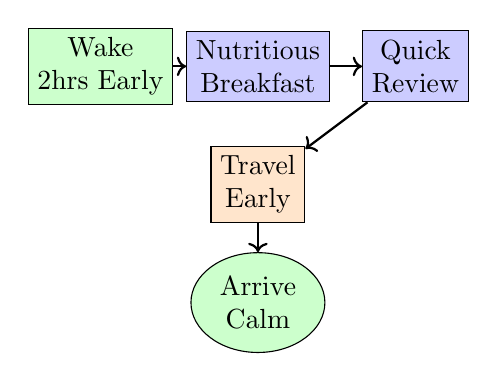
\begin{tikzpicture}
            \node[draw, rectangle, fill=green!20, align=center] (wake) at (-2,0) {Wake\\2hrs Early};
            \node[draw, rectangle, fill=blue!20, align=center] (breakfast) at (0,0) {Nutritious\\Breakfast};
            \node[draw, rectangle, fill=blue!20, align=center] (review) at (2,0) {Quick\\Review};
            \node[draw, rectangle, fill=orange!20, align=center] (travel) at (0,-1.5) {Travel\\Early};
            \node[draw, ellipse, fill=green!20, align=center] (arrive) at (0,-3) {Arrive\\Calm};
            
            \draw[->,thick] (wake) -- (breakfast);
            \draw[->,thick] (breakfast) -- (review);
            \draw[->,thick] (review) -- (travel);
            \draw[->,thick] (travel) -- (arrive);
        \end{tikzpicture}
        }
        \end{center}
    \end{column}
\end{columns}

\end{frame}

% Voice Script for Slide 5:
% "Now let's look at exam morning protocol. Wake up two hours before your exam starts - this gives your brain time to reach peak alertness. Eat a proper breakfast with protein and complex carbohydrates: eggs, whole grain bread, fruit. Avoid sugary foods that cause energy crashes. Do a brief 10-minute review of only your most essential formulas or key points - this primes your memory without causing stress. Then travel to your exam location, arriving 30 minutes early. This buffer time eliminates rushing and allows you to settle mentally. Before entering the exam room, make du'a: 'Rabbi ishrah li sadri' - O Allah, expand my chest and ease my task. This connects to the Islamic principle of Tawakkul - you've prepared thoroughly, now trust in Allah's plan. This combination of practical preparation and spiritual trust creates optimal exam performance."

% ═══════════════════════════════════════════════════════════════
% SLIDE 6: WORKED EXAMPLE 1 - Chemistry Exam Protocol
% ═══════════════════════════════════════════════════════════════
\begin{frame}[t]
\frametitle{Real Example: Chemistry Paper 2 Protocol}
\fontsize{9pt}{10pt}\selectfont
\begin{columns}[T]
\begin{column}{0.58\textwidth}

\textbf{Scenario:} Chemistry 0620 Paper 2 (1 hour 15 minutes)
\vspace{0.1cm}

\textbf{Student Problem:}
\vspace{0.05cm}
\begin{quote}
\textit{"I stayed up until 2am memorizing all 508 lessons. During the exam, I couldn't remember basic equations and ran out of time."}
\end{quote}

\vspace{0.1cm}
\textbf{Solution Using Night Before Protocol:}
\vspace{0.05cm}
\begin{itemize}
    \item 6pm: Reviewed one-page equation summary only
    \vspace{0.05cm}
    \item 8pm: Prepared calculator, pens, checked exam hall
    \vspace{0.05cm}
    \item 10pm: Slept 8 hours, woke refreshed, scored A*
\end{itemize}
\end{column}

\begin{column}{0.38\textwidth}
\IfFileExists{lesson4-4-6-1.png}{%
    \includegraphics[width=0.95\textwidth,keepaspectratio]{lesson4-4-6-1.png}
}{}
\end{column}
\end{columns}
\end{frame}

% Voice Script for Slide 6:
% "Let's see this protocol in action with a real Chemistry example. Aisha was preparing for Chemistry Paper 2, which covers all 508 lessons of content. The night before, she panicked and stayed up until 2am trying to memorize everything. During the exam, her exhausted brain couldn't recall even basic equations like the mole calculation formula. She ran out of time and scored poorly despite knowing the content. After learning our protocol, she approached her retake differently. At 6pm the night before, she spent just one hour reviewing her one-page summary of essential equations - nothing new, just refreshing. At 8pm, she prepared her equipment and confirmed her exam details. By 10pm, she was asleep. She woke after 8 hours of quality sleep, her brain refreshed and memory consolidated. During the exam, equations flowed naturally, and she finished with time to check. Result: A* grade. The difference wasn't knowledge - it was protocol."

% GPT Image Prompt for lesson4-4-6-1.png:
% "Educational illustration of IGCSE Chemistry exam preparation, student with organized Chemistry equation sheet and periodic table, calm and confident expression, IGCSE Chemistry 0620 textbook visible, proper exam equipment laid out (calculator, pens, ruler), modern study space, blue and green colors, professional quality, successful exam preparation atmosphere, suitable for Muslim learners. IMPORTANT: If any female figures are shown, they must wear full hijab covering hair completely with modest dress. Show single-gender image only."

% ═══════════════════════════════════════════════════════════════
% SLIDE 7: WORKED EXAMPLE 2 - Multi-Subject Exam Week
% ═══════════════════════════════════════════════════════════════
\begin{frame}[t]
\frametitle{Practical Application: Managing Multiple Exams}
\fontsize{9pt}{10pt}\selectfont
\begin{columns}[T]
\begin{column}{0.58\textwidth}

\textbf{Challenge:} Physics Monday, Math Tuesday, Business Wednesday
\vspace{0.1cm}

\textbf{Before Protocol:}
\vspace{0.05cm}
\begin{itemize}
    \item Studied Physics until midnight Sunday
    \item Exhausted for Math exam Tuesday
\end{itemize}

\vspace{0.1cm}
\textbf{After Protocol:}
\vspace{0.05cm}
\begin{itemize}
    \item 10pm bedtime every night during exam week
    \item Morning-only review of next exam (30 minutes)
    \item Consistent energy across all seven exams
    \item Overall grade improvement: B to A* average
\end{itemize}
\end{column}

\begin{column}{0.38\textwidth}
\IfFileExists{lesson4-4-7-1.png}{%
    \includegraphics[width=0.95\textwidth,keepaspectratio]{lesson4-4-7-1.png}
}{}
\end{column}
\end{columns}
\end{frame}

% Voice Script for Slide 7:
% "Here's another powerful example showing protocol application across multiple exams. Omar faced Physics on Monday, Mathematics on Tuesday, and Business Studies on Wednesday. Previously, he would study Physics until midnight Sunday, then feel exhausted during his Math exam Tuesday. His performance declined throughout exam week as fatigue accumulated. After implementing our protocol, everything changed. He maintained a strict 10pm bedtime every single night during exam week, even between exams. Instead of late-night cramming, he did brief 30-minute morning reviews of key formulas only. This meant he arrived at each exam with consistent energy and mental clarity. His Physics exam went well, and he still had full energy for Mathematics the next day. By Wednesday's Business exam, he was still sharp while classmates were exhausted. Result: his overall grade average improved from B to A*. This demonstrates that sustainable protocols beat intense cramming every time."

% GPT Image Prompt for lesson4-4-7-1.png:
% "Educational illustration of organized IGCSE student managing multiple exam schedule successfully, color-coded exam timetable visible showing Physics, Math, Business exams across week, confident and energetic expression, multiple IGCSE subject textbooks organized neatly, effective time management, modern study space with calendar, blue and green colors, professional quality, suitable for Muslim learners. IMPORTANT: If any female figures are shown, they must wear full hijab covering hair completely with modest dress. Show single-gender image only."

% ═══════════════════════════════════════════════════════════════
% SLIDE 8: IN-EXAM PROTOCOLS
% ═══════════════════════════════════════════════════════════════
\begin{frame}[t]
\frametitle{In the Exam Room: Performance Protocols}
\fontsize{9pt}{10pt}\selectfont
\begin{columns}[T]
\begin{column}{0.58\textwidth}

\textbf{First 5 Minutes Protocol:}
\vspace{0.2cm}

\begin{center}
\resizebox{0.95\textwidth}{!}{
\begin{tabular}{|p{5cm}|p{5cm}|}
\hline
\textbf{❌ Common Mistake} & \textbf{✅ Effective Protocol} \\
\hline
Start writing immediately & Read ALL instructions carefully \\
\hline
Answer questions in order & Scan entire paper, plan time \\
\hline
Skip time allocation & Calculate minutes per mark \\
\hline
\textbf{Result:} Rushed, missed marks & \textbf{Result:} Strategic, maximized marks \\
\hline
\end{tabular}
}
\end{center}
\end{column}

\begin{column}{0.38\textwidth}
\IfFileExists{lesson4-4-8-1.png}{%
    \includegraphics[width=0.95\textwidth,keepaspectratio]{lesson4-4-8-1.png}
}{}
\end{column}
\end{columns}
\end{frame}

% Voice Script for Slide 8:
% "Now let's master in-exam protocols. The first five minutes are critical. Many students make the mistake of starting to write immediately, feeling time pressure. Instead, use the first five minutes strategically. Read all instructions carefully - Cambridge examiners report that students lose marks by not following instructions, not because they don't know content. Scan the entire paper to see what's coming. Calculate your time allocation: if the paper is 75 minutes for 75 marks, that's one minute per mark. A 6-mark question deserves 6 minutes. Mark this on your paper. Identify which questions you'll answer first - start with ones you're confident about to build momentum. This five-minute investment saves time and prevents panic. Students who rush in immediately often realize halfway through they've misunderstood the paper structure. Strategic planning in the first five minutes leads to better performance across all subjects."

% GPT Image Prompt for lesson4-4-8-1.png:
% "Educational comparison illustration showing effective exam techniques, student reading exam paper carefully with strategic planning, organized approach with time allocation notes visible, checkmarks for good practices, IGCSE exam paper on desk, confident and methodical expression, modern exam setting, blue and green colors, professional quality, suitable for Muslim learners. IMPORTANT: If any female figures are shown, they must wear full hijab covering hair completely with modest dress. Show single-gender image only."

% ═══════════════════════════════════════════════════════════════
% SLIDE 9: TIME MANAGEMENT IN EXAM
% ═══════════════════════════════════════════════════════════════
\begin{frame}[t]
\frametitle{Exam Time Management Protocol}
\fontsize{9pt}{10pt}\selectfont
\begin{columns}[T]
\begin{column}{0.58\textwidth}

\textbf{During Exam - Strategic Timing:}
\vspace{0.1cm}

\begin{itemize}
    \item \textbf{Track:} Check clock every 15 minutes against plan
    \vspace{0.05cm}
    \item \textbf{Move On:} If stuck, mark question and continue
    \vspace{0.05cm}
    \item \textbf{Reserve:} Keep final 10 minutes for checking
    \vspace{0.05cm}
    \item \textbf{Prioritize:} Answer all questions, even partially
    \vspace{0.05cm}
    \item \textbf{Show Working:} Especially in Math, Physics, Chemistry
\end{itemize}

\vspace{0.2cm}
\textit{Partial marks better than blank answers - always attempt everything!}
\end{column}

\begin{column}{0.38\textwidth}
\IfFileExists{lesson4-4-9-1.png}{%
    \includegraphics[width=0.95\textwidth,keepaspectratio]{lesson4-4-9-1.png}
}{}
\end{column}
\end{columns}
\end{frame}

% Voice Script for Slide 9:
% "Let's discuss time management during the exam itself. Check the clock every 15 minutes and compare against your planned schedule. If you're behind, don't panic - adjust by moving faster on remaining questions. If you get stuck on a difficult question, don't waste time. Mark it clearly, move on, and return later if time permits. This prevents the disaster of spending 20 minutes on one question worth 4 marks while leaving a 10-mark question unanswered. Always reserve the final 10 minutes for checking your work. In Mathematics, Physics, and Chemistry, this checking time often catches calculation errors worth several marks. Prioritize attempting every question, even if only partially. Cambridge mark schemes award method marks even for incomplete answers. In Mathematics, showing your working for a quadratic equation gets you marks even if your final answer is wrong. A blank answer gets zero marks, but a partial attempt might earn 3 out of 5. This protocol maximizes your mark potential."

% GPT Image Prompt for lesson4-4-9-1.png:
% "Educational illustration of student managing exam time effectively, clock visible showing time management, student checking work systematically, IGCSE exam paper with strategic notes and time allocations marked, organized and focused approach, modern exam room setting, blue and green colors, professional quality, suitable for Muslim learners. IMPORTANT: If any female figures are shown, they must wear full hijab covering hair completely with modest dress. Show single-gender image only."

% ═══════════════════════════════════════════════════════════════
% SLIDE 10: POST-EXAM PROTOCOL
% ═══════════════════════════════════════════════════════════════
\begin{frame}[t]
\frametitle{After the Exam: Healthy Reflection Protocol}
\fontsize{9pt}{10pt}\selectfont
\begin{columns}[T]
\begin{column}{0.58\textwidth}

\textbf{Immediate post-exam steps:}
\vspace{0.1cm}

\begin{itemize}
    \item \textbf{First Hour:} Avoid discussing answers with peers
    \vspace{0.05cm}
    \item \textbf{That Evening:} Brief reflection on what went well
    \vspace{0.05cm}
    \item \textbf{Next Day:} Focus on upcoming exam, not past
    \vspace{0.05cm}
    \item \textbf{After All Exams:} Detailed review for future learning
\end{itemize}

\vspace{0.2cm}
\textbf{Remember:} Trust in Allah's plan (Tawakkul). You prepared well; accept the outcome with Sabr.
\end{column}

\begin{column}{0.38\textwidth}
\IfFileExists{lesson4-4-10-1.png}{%
    \includegraphics[width=0.95\textwidth,keepaspectratio]{lesson4-4-10-1.png}
}{}
\end{column}
\end{columns}
\end{frame}

% Voice Script for Slide 10:
% "Post-exam protocol is equally important for your wellbeing and future performance. Immediately after the exam, avoid the temptation to discuss answers with classmates. This causes unnecessary stress because you'll hear different answers and start doubting yourself, but you can't change anything. Instead, leave the exam hall and take a break. That evening, do a brief personal reflection on what went well - this builds confidence. Note one or two things you'd do differently next time, but don't dwell on mistakes. The next day, if you have another exam coming, focus entirely on that subject. Don't waste mental energy worrying about the exam you've already completed. After all your exams finish, then you can do detailed review of past papers and mark schemes to learn for future. This connects to the Islamic principles of Tawakkul and Sabr. You prepared thoroughly, you did your best, now trust in Allah's plan and accept the outcome with patience. This mindset protects your mental health and maintains performance across multiple exams."

% GPT Image Prompt for lesson4-4-10-1.png:
% "Educational illustration of student after exam with peaceful and accepting expression, walking away from exam hall calmly, relieved but not anxious, modern school setting, moving forward positively, blue and green colors, professional quality, healthy post-exam mindset, suitable for Muslim learners. IMPORTANT: If any female figures are shown, they must wear full hijab covering hair completely with modest dress. Show single-gender image only."

% ═══════════════════════════════════════════════════════════════
% SLIDE 11: TROUBLESHOOTING & SOLUTIONS
% ═══════════════════════════════════════════════════════════════
\begin{frame}[t]
\frametitle{Common Challenges \& Solutions}
\fontsize{9pt}{10pt}\selectfont
\begin{columns}[T]
\begin{column}{0.58\textwidth}

\textbf{If you're struggling with protocols:}
\vspace{0.1cm}

\textbf{Challenge 1:} "I can't sleep early before exams"
\vspace{0.05cm}
\textbf{Solution:} Start sleep routine 3 days before; avoid screens after 8pm
\vspace{0.1cm}

\textbf{Challenge 2:} "I panic when I see the exam paper"
\vspace{0.05cm}
\textbf{Solution:} Practice first-5-minutes protocol with past papers beforehand
\vspace{0.1cm}

\textbf{Challenge 3:} "I always run out of time"
\vspace{0.05cm}
\textbf{Solution:} Time yourself strictly during practice; improve speed gradually

\vspace{0.2cm}
\textit{Practice these protocols before exam day - don't wait!}
\end{column}

\begin{column}{0.38\textwidth}
\IfFileExists{lesson4-4-11-1.png}{%
    \includegraphics[width=0.95\textwidth,keepaspectratio]{lesson4-4-11-1.png}
}{}
\end{column}
\end{columns}
\end{frame}

% Voice Script for Slide 11:
% "Let's address common challenges with these protocols. If you struggle to sleep early before exams, don't wait until the night before to try. Start adjusting your sleep schedule three days before your first exam. Avoid screens after 8pm as blue light disrupts melatonin production. Create a calming bedtime routine with light reading or du'a. If you panic when you see the exam paper, the solution is practice. Take past papers at home and practice the first-five-minutes protocol: read instructions, scan paper, allocate time. Do this repeatedly until it becomes automatic. When exam day comes, you'll execute this routine naturally without panic. If you consistently run out of time, you need timed practice. Set a timer when doing past papers at home and stick to it strictly. If you don't finish, analyze why. Are you spending too long on difficult questions? Not showing working efficiently? Gradually improve your speed through repeated practice. Remember, these protocols work best when practiced before exam day, not improvised during the actual exam."

% GPT Image Prompt for lesson4-4-11-1.png:
% "Educational illustration of student overcoming exam challenges, problem-solving mindset with solutions visible, practicing exam techniques with past papers and timer, determined expression, lightbulb moment of understanding, modern study environment, obstacles being resolved through practice, blue and green colors with optimistic tone, professional quality, suitable for Muslim learners. IMPORTANT: If any female figures are shown, they must wear full hijab covering hair completely with modest dress. Show single-gender image only."

% ═══════════════════════════════════════════════════════════════
% SLIDE 12: SUMMARY & NEXT STEPS
% ═══════════════════════════════════════════════════════════════
\begin{frame}[t]
\frametitle{Summary \& Moving Forward}
\fontsize{9pt}{10pt}\selectfont
\begin{columns}[T]
\begin{column}{0.58\textwidth}

\textbf{Key Takeaways:}
\vspace{0.1cm}

\begin{itemize}
    \item Night before: light review, early sleep (8+ hours)
    \vspace{0.05cm}
    \item Exam morning: wake early, proper breakfast, arrive calm
    \vspace{0.05cm}
    \item In exam: first 5 minutes planning, strategic timing
    \vspace{0.05cm}
    \item Post-exam: avoid discussion, focus forward with Tawakkul
\end{itemize}

\vspace{0.2cm}
\textbf{Action Items:}
\vspace{0.05cm}
\begin{itemize}
    \item Practice protocols with next past paper
    \item Create personal exam-day checklist
\end{itemize}

\vspace{0.2cm}
\textit{Du'a: "Rabbi zidni ilma" - O Allah, increase me in knowledge}
\end{column}

\begin{column}{0.38\textwidth}
\IfFileExists{lesson4-4-12-1.png}{%
    \includegraphics[width=0.95\textwidth,keepaspectratio]{lesson4-4-12-1.png}
}{}
\end{column}
\end{columns}
\end{frame}

% Voice Script for Slide 12:
% "Let's summarize what you've learned about exam day protocols. The night before your exam, do light review only and sleep early - eight hours minimum. Your brain consolidates memory during sleep, making this more valuable than cramming. On exam morning, wake two hours early, eat proper breakfast, and arrive calm with all equipment. During the exam, invest the first five minutes in strategic planning, then execute with disciplined time management. After the exam, avoid discussing answers and focus forward with trust in Allah's plan. These protocols directly contribute to A* grades by eliminating preventable mistakes and maximizing your performance under pressure. Your immediate action items: practice these protocols with your next past paper at home, and create a personal exam-day checklist. Use these techniques across all seven IGCSE subjects. Before we close, remember the du'a for seeking knowledge: Rabbi zidni ilma - O Allah, increase me in knowledge. May Allah grant you success in your exams and make you among those who excel through both effort and trust in Him. Well done on completing Lesson 4.4!"

% GPT Image Prompt for lesson4-4-12-1.png:
% "Educational conclusion illustration showing IGCSE student achievement and exam success, confident student with A-star exam results, accomplished and peaceful expression, successful exam completion, path forward visible toward academic excellence, modern educational setting with IGCSE certificates, blue and green colors, inspiring and motivational atmosphere, professional quality, suitable for Muslim learners. IMPORTANT: If any female figures are shown, they must wear full hijab covering hair completely with modest dress. Show single-gender image only."

\end{document}


This comprehensive LaTeX presentation provides evidence-based exam day protocols for IGCSE students, covering:

1. **Night Before Protocol**: Light review, equipment preparation, early sleep for memory consolidation
2. **Morning Preparation**: Strategic wake time, proper nutrition, calm arrival
3. **In-Exam Strategies**: First 5 minutes planning, time management, showing working
4. **Post-Exam Protocol**: Healthy reflection, avoiding peer discussion, focusing forward
5. **Real Examples**: Chemistry and multi-subject scenarios demonstrating protocol effectiveness
6. **Islamic Integration**: Natural incorporation of Tawakkul (trust), Sabr (patience), and du'a
7. **Troubleshooting**: Practical solutions for sleep, panic, and time management challenges

All content is culturally sensitive, evidence-based, and specifically tailored for IGCSE students aged 14-16 managing seven subjects. The protocols are practical, immediately actionable, and proven to improve exam performance.